\chapter{Asservissement visuel} \label{chap1}

La vision représente pour les humains environ 70\% des données issues des 
perceptions sensorielles externes \cite{purves2004neuroscience} : d'une 
richesse incroyable, c'est aussi, par conséquent, une source d'erreurs 
inépuisable. La vision artificielle ne déroge pas à ses deux principes, d'où 
l'importance du traitement du signal d'une part (dans le but de recueillir et 
interpréter dans cette grande variété d'informations ce qui est pertinent pour 
une tâche prescrite) et d'une stratégie d'asservissement d'autre part (afin de 
stabiliser une tâche malgré les erreurs et incertitudes sur les données).

Nous allons donc dans un premier temps présenter le mode d'acquisition des 
images, puis nous continuerons sur les modèles de perception utilisés. Une fois 
que nous aurons détaillé la manière dont une scène est projetée sur une image, 
nous pourrons dans une seconde section distinguer plusieurs configurations et 
exposer différentes stratégies d'asservissement pouvant être utilisées. Une 
troisi\`eme section sera consacr\'ee \`a la construction des lois de 
commandes, dont nous fournirons quelques exemples. La quatri\`eme section de ce 
chapitre pr\`esentera les sp\'ecificit\'es d'une utilisation de 
l'asservissement visuel dans le contexte des maipulateurs parall\`eles \`a 
c\^ables : apr\`es avoir pr\'esent\'e les principaux travaux ayant \'et\'e 
effectu\'es dans ce domaine, nous pourrons indiquer les angles d'\'etudes que 
nous avons privil\'egi\'es, les probl\'ematiques aui en \'emergent, et les 
pistes de r\'esolution que nous avons emprunt\'ees.
 
\section{Modèles de capteurs et projections} \label{chap1-0}
 
\subsection{De l'oeil à la caméra} \label{chap1-0-0}
 
Sans pour autant chercher à imiter la vision humaine, la vision artificielle 
s'en inspire néanmoins fortement pour ce qui concerne l'acquisition d'une 
image. Ainsi, pour une caméra, le diaphragme joue le rôle de l'iris et de la 
pupille et détermine la quantité de lumière qui pourra être enregistrée sur un 
intervalle de temps donné. Par la suite, la lentille joue un rôle équivalent à 
la cornée et au cristallin, en faisant converger les rayons lumineux vers la 
rétine sur laquelle sont disséminés environ 125 millions de photorécepteurs : 
c'est au niveau de ces derniers que l'acquisition est véritablement effectuée. 
On distingue parmi les photorécepteurs :
 \begin{figure}[htp]
  \centering
  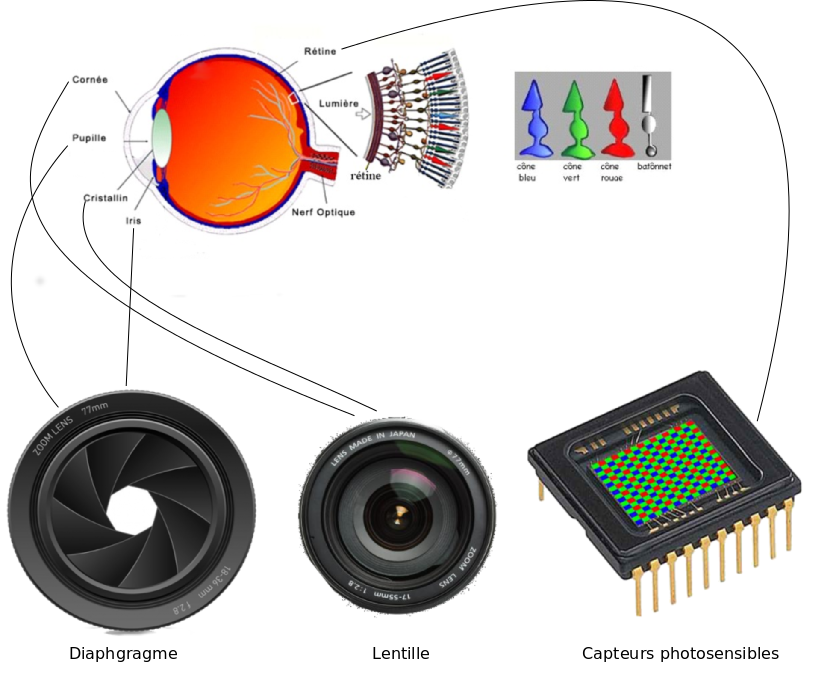
\includegraphics[width=.85\linewidth]{./chapter01/figures/oeil.png}
    \caption{\footnotesize{Oeil humain vs vision artificielle}}
\label{chap01:fig01}
\end{figure}

 \begin{itemize}
  \item les cônes, généralement impliqués dans la vision diurne. Les cônes 
présen\-tent 3 types de pigments leur permettant de réagir à des longueurs 
d'ondes spécifiques (qui ne recouvrent pas exactement le triplet RGB 
traditionnellement utilisé en traitement d'image)
  \item les bâtonnets, impliqués dans la vision nocturne. Ne possédant qu'un 
seul type de pigments, ils ne peuvent pas discriminer les longueurs d'ondes. En 
revanche, ils sont en moyenne 1000 fois plus sensibles à la lumière que les 
cônes, et leur population correspond à 20 fois celle des cônes.
 \end{itemize}

Afin de simuler l'activité des photorécepteurs de l'oeil humain, les 
dispositifs technologiques les plus récents adoptent des stratégies basées sur 
l'utilisation de filtres placés en amont des capteurs photosensibles, 
permettant 
ainsi une acquisition en séquence (un même récepteur recevra successivement les 
réponses des filtres correspondants aux longueurs d'ondes distinguées) ou 
simultanée (les réponses sont envoyées sur des capteurs photosensibles dédiés).
  
L'information contenue dans les données ainsi recueillies est riche et multiple 
: elle peut-être de nature colorimétrique, géométrique, elle permet de 
ca\-ractériser des déplacements, des déformations. Toutefois, ce qui est vu 
n'est jamais qu'une représentation de ce qui est observé : il est d\`es lors 
fondamental d'exploiter les donn\'ees recueillies de mani\`ere \`a tendre 
vers une repr\'esentation exploitable de la scène initiale projetée sur les 
capteurs.

Une premi\`ere option serait de tenter de reconstruire la sc\`ene le plus 
fid\`element possible. On pourra dans ce cas privil\'egier l'utilisation de 
cam\'eras st\'er\'eos (Fig.\ref{chap01:fig02view0})\cite{brandou2006}, ou encore de capteurs RGB-D (Fig.\ref{chap01:fig02view1})\cite{siradjuddin2012}. A l'aide de cam'eras st\'er\'eos, nous pouvons percevoir la sc\`ene selon plusieurs perspectives, 
tout comme avec la vision binoculaire. En croisant les donn\'ees obtenues \`a 
partir des diff\'erents points de vue, il est possible d'approcher une 
repr\'esentation tri-dimensionnelle de la sc\`ene acquise au sein de l'image. 
Quant aux capteurs RGB-D, ils compl\`etent les donn\'ees acquises gr\^ace \`a 
une ou plusieurs cam\'eras avec de dispositifs permettant de recueillir une 
information sur la profondeur. La fusion des donn\'ees g\'eom\'etriques et 
colorim\'etriques obtenues par les cam\'eras classiques et de la localisation 
tridimensionnelle de points permet une reconstruction 3D de la sc\'ene 
observable. En multipliant les points de vue (soit par le mouvement, soit en 
utilisant plusieurs dispositifs), ou en exploitant un mod\`ele connu de la 
sc\`ene observ\'e, on sera en mesure d'obtenir une repr\'esentation fid\`ele 
d'un environnement. Ce sont toutefois des dispositifs on\'ereux, qui peuvent 
sembler inutilement intrusifs selon le contexte d'utilisation, et requ\'erant 
bien souvent une puissance de calcul d\'emesur\'ee par rapport aux informations 
dont on a besoin.

\begin{figure}[!ht]
  \centering
      \subfloat[Jean-Luc Godard exp\'erimentant avec la st\'er\'eographie pour tourner {\it Adieu au langage 3D}]{\label{chap01:fig02view0}
    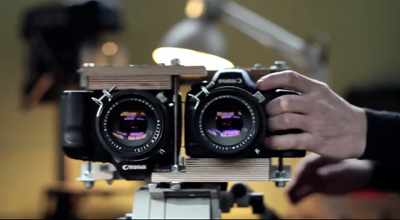
\includegraphics[width=.54\linewidth]{./chapter01/figures/stereo_godard.jpg}} 
\hfill
    \subfloat[La Kinect de @Microsoft qui a permis la d\'emocratisation de l'utilisation des capteurs RGB-D]{\label{chap01:fig02view1}
    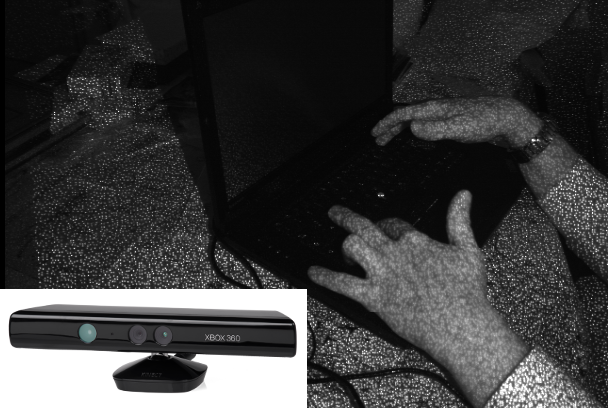
\includegraphics[width=.44\linewidth]{./chapter01/figures/kinect.png}}
    \caption{\footnotesize{Exemples de cam\'eras st\'er\'eo et de capteurs RGB-D.}}
\label{chap01:fig02}
\end{figure}

Une seconde option est de d\'eterminer les transformations g\'eom\'etriques d'objets dans le plan image g\'en\'er\'ees par une modification soit d'une partie de la sc\`ene (objet en mouvement), soit de la pose de la cam\'era elle-m\^eme, voire des deux simultan\'ement. Ceci permet entre autres de s'abstraire en partie au moins de la repr\'esentation tridimensionnelle de la sc\`ene projet\'ee sur l'image, en utilisant par exemple la g\'eom\'etrie pl\"uckerienne \cite{andreff:inria-00072393}, des descripteurs locaux ou globaux \cite{latuan2010}, des repr\'esentations fr\'equentielles (Fourier \cite{chari2008}, ondelettes \cite{ramosvelasco2012}), $\cdots$ (on pourra retrouver les principales techniques dans \cite{marchand2005}).

Le choix d'un type de capteur n'est donc pas anodin, il d\'epend de param\`etres aussi divers que la quantit\'e et la densit\'e des informations, les connaissances pr\'ealables que l'on peut avoir d'une sc\`ene ou d'un objet, du type d'informations disponibles dans l'images et pertinentes par rapport au contexte (sc\`enes homog\`enes ou textur\'ees, mobiles ou statiques, diurnes ou nocturnes, $\cdots$).

Nous partirons du principe que nous utilisons une seule cam\'era simple, ce choix \'etant justifi\'e dans la derni\`ere section de ce chapitre. L'objectif est \`a pr\'esent de d\'efinir le mod\`ele de repr\'esentation que nous avons utilis\'e, soit la mani\`ere dont la sc\`ene est projet\'ee dans l'image.

\subsection{De la scène à l'image} \label{chap1-0-1}

\subsubsection{Mod\`ele de projection} \label{chap1-0-1-0}

Nous avons privilégié le modèle {\it pinhole} qui offre une approximation 
fiable des caméras perspectives (telles que celles que nous avons utilisées) 
tout en restant formellement simple \cite{Faugeras:1993} \cite{hartley2004}, 
sous les hypothèses du respect des conditions de Gauss (angles de faibles 
incidences), et -- c'est notre cas -- d'une absence de distorsion de la caméra.

Soient ${\bf P} = (X, Y, Z)$ les coordonnées 3-D d'un point dans l'espace et 
${\bf p} = (x_m, y_m)$ ses coordonnées m\'etriques dans l'image. Le modèle de 
projection perspective consiste en une projection centrale de centre $\mathcal 
C$, portée par l'axe ${\bf z}_c$ représentant l'axe optique de la caméra. On 
appelle {\it plan image} le plan se trouvant à distance focale $f$ de la 
caméra, 
soit $Z = f$. On définit également un point de référence ${\bf c}(x_c,y_c)$ 
dans 
le plan image comme étant le point d'intersection de l'axe optique et du plan 
image (Fig.\ref{intro:fig12}).

\begin{figure}[h!tp]
  \centering
  \def\svgwidth{.85\linewidth}
  \input{./chapter01/figures/modele_projection.pdf_tex}
    \caption{\footnotesize{Modèle de projection {\it pinhole}}}
\label{intro:fig12}
\end{figure}

En plus du {\it référentiel-base} $\mathcal R_b$ et du r\'ef\'erentiel de 
l'organe terminal $\mathcal R_e$ (cf. Section \ref{}) s'ajoutent un 
%rajouter reference
{\it référentiel-caméra} noté $\mathcal R_c$, un {\it référentiel-objet} 
$\mathcal R_o$, ainsi qu'un {\it référentiel-image} $\mathcal R_i$. Nous 
noterons également $l_x$ et $l_y$ respectivement la longueur et la hauteur d'un 
pixel dont nous aurons besoin pour la suite.

A partir des coordonnées d'un point ${\bf P}(X, Y, Z)$ exprimées dans le 
référentiel de la caméra, les coordonnées projetées sur le plan images sont 
déduites de la manière suivante :

\begin{equation}
x_m = f \frac{X}{Z}, y_m = f \frac{Y}{Z}
\label{intro:eq12}
\end{equation}

ou, sous forme matricielle :

\begin{equation}
Z
\begin{bmatrix}
x_m \\y_m \\ 1
\end{bmatrix}
=
\begin{bmatrix}
f & 0 & 0 \\ 0 & f & 0 \\ 0 & 0 & 1 
\end{bmatrix}
\begin{bmatrix}
X \\ Y \\ Z 
\end{bmatrix}
\label{intro:eq13}
\end{equation}
soit $\widetilde {\bf p} = {\bf A}{\bf P}$, avec $\widetilde {\bf p} = Z {\bf 
p}$.

Un point dans l'image est généralement représenté par ses coordonnées 
pi\-xelliques (l'origine du référentiel étant supposée localisée en haut à 
gauche de l'image).

La conversion entre les coordonnées métriques $(x_m, y_m)$ et les coordonnées 
pixelliques $(x_p, y_p)$, se fait selon la relation suivante :

\begin{equation}
\left \lbrace
\begin{matrix}
x_p = x_c + x_m/l_x \\
y_p = y_c + y_m/l_y
\end{matrix} \right .
\label{intro:eq14}
\end{equation}
ce qui donne sous une forme matricielle :

\begin{equation}
\begin{bmatrix}
x_p \\y_p \\ 1
\end{bmatrix}
=
\begin{bmatrix}
\frac 1 {l_x} & 0 & x_c \\ 0 & \frac 1 {l_y} & y_c \\ 0 & 0 & 1 
\end{bmatrix}
\begin{bmatrix}
x \\ y \\ 1
\end{bmatrix}
\label{intro:eq15}
\end{equation}
soit ${\bf p}_p = {\bf B} {\bf p}$.

On obtient la relation suivante entre les coordonnées métriques 3-D du point et 
les coordonnées pixelliques dans l'image :
\begin{equation}
Z\begin{bmatrix}
x_p \\y_p \\ 1
\end{bmatrix}
=
\begin{bmatrix}
\alpha_x & 0 & x_c \\ 0 & \alpha_y & y_c \\ 0 & 0 & 1 
\end{bmatrix}
\begin{bmatrix}
X \\ Y \\ Z
\end{bmatrix}
\label{intro:eq16}
\end{equation}
avec $\alpha_x = f/l_x$ et $\alpha_y = f/l_y$. Les paramètres $(\alpha_x, 
\alpha_y, x_c, y_c)$ de la matrice ${\bf K} = {\bf A}{\bf B}$ ainsi construite 
sont généralement obtenus par calibration \cite{brown71}, \cite{tsai1986}, 
\cite{stein1997}. La matrice ${\bf K}$ nous permet de faire le lien entre les 
informations géométriques disponibles dans l'image et la projection de la scène 
observée. En particulier, nous pouvons à présent définir les 
coordonnées normalisées ainsi :
\begin{equation}
\left \lbrace
\begin{matrix}
x = X/Z \\
y = Y/Z
\end{matrix} \right .
\label{intro:eq17}
\end{equation}
indépendantes de la focale, et pouvant être déduites des coordonnées 
pixelliques en utilisant la matrice $\bf K$.

Enfin, les coordonn\'ees 3D du point \'etant exprim\'ees dans le rep\`ere cam\'era, nous voulons pouvoir les traduire dans le r\'ef\'erentiel propre de l'objet.

\subsubsection{Changements de rep\`ere} \label{chap1-0-1-1}

Soient \`a pr\'esent ${}^c{\bf P} = ({}^cX, {}^cY, {}^cZ)$ les coordonnées du point ${\bf P}$ 
exprimées dans le référentiel $\mathcal R_c$ et ${}^o{\bf P} = ({}^oX, {}^oY, 
{}^oZ)$ ses coordonnées dans le référentiel $\mathcal R_o$. Le passage d'un 
référentiel à l'autre est effectué en utilisant la relation ${}^c{\bf P} = 
{}^c{\bf t}_o + {}^c{\bf R}_o {}^o{\bf P}$, avec ${}^c{\bf t}_o$ le vecteur 
$3\times 1$ de translation entre les deux référentiels, ${}^c{\bf R}_o$ la 
matrice $3\times 3$ de rotation correspondant à la rotation autour des axes du 
référentiel. En utilisant les coordonnées homogènes $\widetilde {\bf P}$ de 
${\bf P}$, il est possible de factoriser cette transformation en une seule 
opération matricielle :
\begin{equation}
{}^c \widetilde {\bf P} = {}^c {\bf M}_o {}^o \widetilde {\bf P}
\label{intro:eq18}
\end{equation}
soit :
\begin{equation}
\begin{bmatrix}
{}^cX \\ {}^cY \\ {}^cZ \\ 1
\end{bmatrix}
=
\begin{bmatrix}
&  {}^c{\bf R}_o & & {}^c{\bf t}_o \\
& {\bf 0} & & 1
\end{bmatrix}
\begin{bmatrix}
{}^oX \\ {}^oY \\ {}^oZ \\ 1
\end{bmatrix}
\label{intro:eq19}
\end{equation}

On appelle ${}^c{\bf M}_o$ la {\it matrice homogène de transformation} du 
référentiel $\mathcal R_o$ au référentiel $\mathcal R_c$, dont l'inverse 
s'exprime simplement sous la forme :
\begin{equation}
{}^o{\bf M}_c = 
\begin{bmatrix}
&  {}^c{\bf R}_o^T & & -{}^c{\bf R}_o^T {}^c{\bf t}_o \\
& {\bf 0} & & 1
\end{bmatrix}
\label{intro:eq20}
\end{equation}

Nous sommes dès lors en mesure d'établir une relation entre la scène observée 
dans son référentiel propre, dans le r\'ef\'erentiel de la cam\'era (et par extension dans chacun des r\'ef\'erentiels du manipulateur) et sa projection dans l'image, exprimée en coordonnées pixelliques, métriques et normalisées. Le lecteur 
remarquera cependant que, s'il est possible directement, connaissant ${\bf K}$ 
et ${}^o{\bf M}_c$, de déduire à partir des propriétés de la scène les 
caractéristiques de sa projection, l'opération inverse est dépendante dans ce 
modèle d'une estimation pour chaque point de sa profondeur (coordonnée ${}^cZ$), ce dont nous aurons \`a tenir compte lorsqu'il s'agira de d\'eterminer le type de mesure que nous utiliserons pour d\'eduire les consignes donn\'ees au manipulateur.

\section{Modalit\'es d'asservissement visuel} 
\label{chap1-1}



\subsection{Positionnement de la caméra} \label{chap1-1-0}

Le contexte étant celui d'un manipulateur dont on veut asservir la saisie et le déplacement d'un objet, plusieurs stratégies s'offrent 
à nous. Une première décision à prendre concerne par exemple le positionnement 
de la caméra. On distingue ainsi une configuration déportée 
(Fig.\ref{intro:fig13view0}) d'une configuration embarquée (Fig. 
\ref{intro:fig13view1}).

\begin{figure}[htp]
  \centering
  \subfloat[La caméra est déportée ; la scène comprend l'organe terminal et 
l'objet-cible]{\label{intro:fig13view0}
    \def\svgwidth{.45\linewidth}
  \input{./chapter01/figures/eye_to_hand.pdf_tex}} \hfill
    \subfloat[La caméra est embarquée ; la scène ne comprend que 
l'objet-cible]{\label{intro:fig13view1}
    \def\svgwidth{.45\linewidth}
  \input{./chapter01/figures/eye_in_hand.pdf_tex}} 
    \caption{\footnotesize{Positionnements de caméra}}
\label{intro:fig13}
\end{figure}

Dans le cas d'une caméra déportée fixe, il est possible d'avoir une approximation des transformations permettant de 
passer du référentiel-base $\mathcal R_b$ au référentiel-caméra $\mathcal R_c$, 
et du référentiel-caméra au référentiel-objet $\mathcal R_o$. Seul l'organe 
terminal bouge dans la scène observée. Dans le cas d'une caméra embarquée, la 
transformation permettant de passer du référentiel de l'organe terminal 
$\mathcal R_e$ au référentiel-caméra $\mathcal R_c$ est connue. Toutefois, 
l'ensemble de la scène est affecté lors d'un déplacement de l'organe terminal 
(et donc de la caméra).

\subsection{Asservissements en position, basés images et hybrides} 
\label{chap1-1-1}

De manière générale, une stratégie d'asservissement visuel peut être décomposée 
de la manière suivante :
\begin{enumerate}
 \item on sélectionne dans un premier temps un ensemble ${\bf s}$ de paramètres 
à partir desquels on peut estimer soit directement la pose de l'organe 
terminal, 
soit le déplacement nécessaire à l'obtention de cette pose. L'ensemble des 
paramètres dépend d'une part de la valeur des primitives extraites de l'image 
et 
d'autre part d'un ensemble de connaissances {\it a priori}, telles que les 
propriétés de la caméra, ou encore un modèle de la cible.
 \item on définit ensuite la valeur désirée ${\bf s}^*$ des paramètres, 
correspondant à l'état que l'on souhaite atteindre.
 \item à partir de données extraites de l'image, on calcule la valeur courante 
des paramètres
 \item on calcule alors une erreur ${\bf e} = {\bf s} - {\bf s}^*$, dont on 
souhaite qu'elle converge vers $0$.
 \item on établit enfin une relation entre la variation $\dot {\bf e}$ de 
l'erreur et la commande qui sera ensuite envoyée au manipulateur.
 \item la commande est effectuée, et l'on boucle les étapes $3$ à $6$ jusqu'à 
obtention d'une valeur seuil de l'écart entre les valeurs courantes des 
paramètres et les valeurs désirées.
\end{enumerate}

\begin{figure}[htp]
  \centering
    \def\svgwidth{.95\linewidth}
  \input{./chapter01/figures/bloc_commande.pdf_tex}
    \caption{\footnotesize{Schéma des étapes de l'asservissement visuel}}
\label{intro:fig13b}
\end{figure}

On distinguera ici deux grandes classes de stratégies d'asservissement : la 
première est basée sur l'estimation des paramètres de pose de l'organe terminal 
(PBVS : position-based visual servo), tandis que la seconde utilise directement 
les primitives extraites de l'image (IBPS : image-based visual servo). Il est 
également possible de mixer ces deux approches, ce que l'on appellera un 
asservissement hybride.

Dans le cas de l'asservissement en position, une connaissance du modèle 3-D de 
la cible est nécessaire (on parle d'ailleurs parfois d'asservissement 3-D). De 
l'écart entre les valeurs courantes d'un ensemble de primitives et leurs 
valeurs 
estimées pour une pose désirée, on déduira les paramètres de pose de l'organe 
terminal. Cela revient à faire varier un référentiel courant de l'organe 
terminal $\mathcal R_e$ vers un référentiel correspondant à la pose prescrite 
$\mathcal R_e^*$, soit la détermination d'une matrice homogène de 
transformation 
${}^{e^*}{\bf M}_e$. Comme nous l'avons vu, cette matrice est composée d'une 
translation et d'une rotation, qui peuvent être décrites à l'aide de $6$ 
paramètres. Dans ce cas, le vecteur ${\bf s}$ est constitué de mesures 
permettant de construire cette matrice de transformation de repère. On pourra 
d'ailleurs noter que dans une configuration avec caméra embarquée, le problème 
est équivalent à la détermination d'une matrice de transformation ${}^{c^*}{\bf 
M}_c$ entre les référentiels courants et désirés de la caméra.

L'asservissement basé-image repose quant à lui sur l'exploitation direct des 
informations extraites de l'image pour établir la commande qui sera envoyée au 
manipulateur. Il ne nécessite pas de connaissance {\it a priori} du modèle 3-D 
de l'objet, mais exploite des primitives pour lesquelles on possède un modèle 
de 
comportement lorsqu'elles évoluent dans l'espace. On parlera dès lors 
d'asser\-vissement 2-D, ou d'asservissement 2-D 1/2 lorsque une connaissance du 
modèle 3-D est néanmoins utilisée (approche hybride).

Quelque-soit la situation, l'objectif de l'asservissement visuel est de 
traduire 
un ensemble de mesures effectuées dans une série d'image en loi de commande qui 
sera envoyée au manipulateur.

\subsection{Construction d'une loi de commande}\label{chap1-1-2}

Nous reprenons ici les bases de construction d'une loi de commande 
\cite{samson1991}. Le lecteur les retrouvera développées par exemple dans 
\cite{chaumette:tuto01} et \cite{chaumette:tuto02}. Nous nous contentons ici 
d'exposer les principes généraux d'outils que nous avons utilisés tout au long 
de nos travaux.

Soient ${\bf s}$ un ensemble de mesures réalisées au sein de l'image sur des 
primitives choisies, et ${\bf s}^*$ les valeurs désirées de ces mesures. On 
construit le vecteur ${\bf e} = {\bf s} - {\bf s}^*$ représentant l'erreur de 
mesure, soit la différence entre les valeurs courantes et les valeurs désirées.

On choisit ici de construire une loi de commande en vitesse. Soit le torseur 
cinématique ${\bf v}_c = ({\bf \nu}_c, {\bf \omega}_c)$, avec ${\bf \nu}_c$ et 
${\bf \omega}_c$ les vitesses instantanées respectivement linéaires et 
angulaires. Il est nécessaire dans un premier temps de déterminer les 
variations $\dot {\bf s}$ des mesures pour un déplacement donné ${\bf v}_c$ de 
la caméra. Cette relation, lorsqu'elle existe, prend la forme algébrique d'une 
matrice ${\bf L}_s \in \mathcal M_{k\times 6}$ que l'on appelle {\it matrice 
d'interaction} \cite{espiau1992}, $k$ représentant le nombres de mesures 
effectuées. A partir de tous ces éléments nous pouvons établir :

\begin{equation}
\dot {\bf s} = {\bf L}_s {\bf v}_c
\label{intro:eq21}
\end{equation}

Notre cible étant fixe, nous avons $\dot {\bf e} = \dot {\bf s}$. Nous pouvons 
dès lors immédiatement déduire de (Equ.\ref{intro:eq21}) la relation suivante :
\begin{equation}
\dot {\bf e} = {\bf L}_e {\bf v}_c
\label{intro:eq22}
\end{equation}

Nous souhaitons que notre erreur ${\bf e}$ de mesure décroisse de manière 
exponentielle, soit : $\dot {\bf e} = - \lambda {\bf e}$, $\lambda$ étant 
appelé 
le {\it gain}, permettant de régler la vitesse de convergence. La loi de 
commande suivante peut alors être construite :
\begin{equation}
{\bf v}_c = - \lambda {\bf L}_e^+ {\bf e} 
\label{intro:eq23}
\end{equation}
où ${\bf L}_e^+ \in \mathcal M_{6 \times k}$ représente la matrice 
pseudo-inverse de Moore-Penrose, soit ${\bf L}_e^+ = ({\bf L}_e^T {\bf 
L}_e)^{-1} {\bf L}_e^T$. Lorsque $k = 6$ et que $\det {\bf L}_e \neq 0$, on 
pourra choisir d'utiliser la loi ${\bf v}_c = - \lambda {\bf L}_e^{-1} {\bf e} 
$.

En pratique, il est difficile de connaître avec exactitude ${\bf L}_e$, qui 
peut 
être dépendante de la pose de la caméra. On utilisera dès lors une 
approximation 
de la matrice d'interaction, la loi de commande finale devenant :
\begin{equation}
{\bf v}_c = - \lambda \widehat {{\bf L}_e^+} {\bf e} 
\label{intro:eq24}
\end{equation}

Toutes les fois où cela est possible, on préfèrera utiliser des primitives dont 
la matrice d'interaction correspondante exhibe des propriétés algébriques 
inté\-ressantes (triangulaire, inversible, \dots). Le choix préalable des 
primitives obéit donc à un double impératif :
\begin{itemize}
 \item on attend qu'elles soient aisément identifiables dans l'image et que les 
mesures puissent être réalisées de manière robuste
 \item les caractéristiques de la matrice d'interaction qu'elles complètent 
doivent comporter des qualités algébriques qui permettront d'améliorer les 
calculs tout autant que de ne pas propager les erreurs de mesures sur une 
primitive particulière aux autres mesures.
\end{itemize}


\section{Contexte de l'étude et choix de stratégie pour l'asser\-vissement 
visuel}\label{chap1-2}

Nous avons vu que l'utilisation d'un robot parallèle à câbles nous permet 
d'évoluer dans un espace de travail conséquent. En particulier, le robot {\tt 
Marionet-Assist} que nous avons utilisé pour nos expérimentations évolue dans 
un cube de $4m \times 3m \times 3m$, et le volume atteignable par un robot de type 
{\tt Marionet-Crane} peut aller jusqu'à $100m \times 35m \times 35m$. Dans ces 
circonstances, l'utilisation d'une caméra embarquée a été privilégiée pour deux 
raisons :
\begin{itemize}
 \item le champs de vision d'une seule caméra fixe déportée pourra se révéler 
insuffisant pour couvrir l'ensemble de l'espace de travail
 \item le déploiement d'un robot à câble pouvant être effectué dans des milieux 
nocifs, ou difficilement atteignables (suite par exemple à une catastrope 
naturelle), l'utilisation d'une caméra déportée est souvent difficilement 
envisageable.
\end{itemize}

Ajoutons que le robot {\tt Marionet-Assist} a été pensé pour être utilisé dans 
des pièces de vie de personnes à la mobilité fragilisée. Dans ce cadre, une 
caméra déportée peut paraître inutilement intrusive. Le champs de vision d'une 
caméra embarquée étant limité, cela nous a semblé, conformément à cette 
application, un choix plus respectueux de l'intimité des personnes. 

De la même manière, les environnements d'utilisation des robots à câbles de la 
famille {\tt Marionet} sont généralement dynamiques. A ce titre, nous avons 
privilégié une stratégie d'asservissement basé-image, à nouveau pour deux 
raisons distinctes :
\begin{itemize}
\item elle ne nécessite pas une connaissance complète du modèle 3-D de la cible 
\item l'asservissement en position repose souvent sur l'utilisation de 
plusieurs 
caméras (ou de capteurs de type RGB-D) pour garantir une mesure fiable des 
primitives permettant une reconstruction du modèle 3-D de la cible. Or, pour 
des 
raisons toujours liées au contexte d'application des robots de la famille {\tt 
Marionet}, cela ne correspond pas aux choix de capteurs que nous avons effectués
\end{itemize}

Enfin, il était envisageable dans cette étude d'utiliser les caméras soit comme 
capteur intéroceptif, soit comme capteur extéroceptif. Le choix d'une 
observation des articulations d'un robot parallèle à câbles a été effectué par 
\cite{andreff2007} pour des robots parallèles classiques, et plus récemment 
pour 
des robots parallèles à câble \cite{dallej2011}, \cite{dallej2012}. Ces études 
correspondant à ce jour au principal travail effectué dans le domaine de 
l'asservissement visuel des robots parallèles à câbles, nous reviendrons dès 
lors dessus à l'occasion de la section suivante, au sein de laquelle nous 
définirons nos problématiques et pistes de travail. Nous pouvons relever 
toutefois que la démarche développée dans leurs recherches consiste à améliorer 
le positionnement de l'organe terminal, ce qui suppose que la position de la 
cible est connue avec suffisamment de précision. Il s'agit donc d'un 
environnement contrôlé. Or, le contexte d'application de nos robots implique au 
contraire une incertitude non-négligeable sur les propriétés de la cible. Dès 
lors, la caméra est tout autant utilisée pour la construction d'une loi de 
commande que pour la localisation de l'objet et l'actualisation de ses 
propriétés lorsque celles-ci diffèrent d'une première estimation. Le choix 
d'utilisation des caméras comme capteurs extéroceptifs s'est donc imposé dans 
notre approche.

Il nous reste en introduction à présenter les avantages et les spécificités 
d'une utilisation de l'asservissement visuel dans le contexte particulier des 
robots parallèles à câbles. La section suivante introduira les pistes 
d'amélioration de contrôle que nous avons repérées, les problématiques 
auxquelles nous avons été confrontées et la manière dont nous proposons de les 
résoudre. Nous évoquerons également de quelle manière les spécificités des 
robots parallèles nous permettent d'assouplir les contraintes de 
l'asservissement tout en garantissant un contrôle optimal.

\section{Asservissement visuel des robots parallèles à 
câbles}\label{chap1-3}

Nous avons vu que plusieurs caract\'eristiques des robots parall\`elles
\`a c\^ables peuvent alt\'erer la qualit\'e de la manipulation. Ainsi, la
complexit\'e des mod\`eles g\'eom\'etriques et cin\'ematiques par rapport aux
robots s\'eries et aux robots parall\`eles rigides menace d'une part la
pr\'ecision des op\'erations de manipulation lors de la r\'esolution
num\'erique, et d'autre part l'effectuation en temps r\'eel. De plus, la
n\'ecessaire v\'erification de l\'equilibre statique pour toutes les
configurations de c\^ables en tension strictement positive impacte \'egalement
la contrainte de r\'ealisation en temps r\'eel d'une t\^ache ; surtout, il est
tout autant difficile de pr\'evoir quels c\^ables seront en tension lors d'un
d\'eplacement prescrit, que de garantir la constance du caract\`ere positif ou
nul de la tension d'un c\^able sur l'int\'egralit\'e d'un d\'eplacement. Enfin,
les incertitudes m\'ecaniques -- telles par exemple le diam\`etre r\'eel de la
couche d'enroulement d'un c\^able autour des tambours -- ont \'egalement une
influence sur la pr\'ecision du manipulateur.

Il est donc n\'ecessaire, afin de garantir l'efficacit\'e d\'une t\^ache de
manipulation, de simplifier la r\'esolution num\'erique des mod\`eles, de
d\'evelopper une strat\'egie de contr\^ole de la tension dans les diff\'erents
c\^ables, et de corriger enfin la trajectoire du manipulateur lorsque les
incertitudes et erreurs perturbent celle-ci.

L'utilisation de capteurs suppl\'ementaires a \'et\'e propos\'ee \`a de
nombreuses reprises afin de r\'esoudre un ou plusieurs des probl\`emes
\'enonc\'es. Dans le contexte des robots parall\`eles \`a jambes rigides,
plusieurs suggestions ont \'et\'e faites :
\begin{itemize}
 \item mesurer directement la pose de l'organe terminal \`a l'aide de
syst\'emes de lasers et miroirs \cite{marantette1995machine}, \cite{Heeren:1992}
ou d'une cam\'era d\'eport\'ee \cite{dallej.2006}, \cite{paccot.2008} : cela
permet tout autant une simplification des mod\`eles qu'une correction des
erreurs et impr\'ecisions.
\item utiliser des capteurs proprioceptifs afin d'obtenir une repr\'esentation
fid\`ele de l'\'etat des variables articulaires
\cite{merlet.1993}, \cite{parenti.2000}, ce qui permet \'egalement une
simplification des mod\`eles pouvant aboutir \`a une ex\'ecution en temps
r\'eel. 
\item un contr\^ole r\'ef\'erenc\'e vision bas\'e sur l'exploitation de mesures
des directions des jambes du robot \cite{andreff2007} : dans cette derni\`ere
m\'ethode, une strat\'egie IBVS est utilis\'ee pour d\'efinir un contr\^ole
cin\'ematique. Elle permet de s'affranchir du calcul du MGD, ce qui la rend
{\it a priori} robuste aux erreurs de mod\`eles et de calibrations.
\end{itemize}

En particulier, cette derni\`ere m\'ethode a \'et\'e d\'eclin\'ee r\'ecemment
pour le contr\^ole de robots parall\`eles \`a c\^ables. Elle fait suite \`a
une premi\`ere approche \cite{conf/iros/DallejGAMM11} consistant \`a mettre dans
un premier temps en place un asservissement visuel 3-D (PBVS) sur l'organe
terminal, puis \`a \'elaborer un sch\'ema de contr\^ole dynamique utilisant la
vision pour estimer la pose et la v\'elocit\'e de la plate-forme. Malgr\'e des
r\'esultats prometteurs obtenus en simulation, il reste \`a valider cette
approche sur un prototype r\'eel.

Les m\^emes auteurs ont donc par la suite propos\'e une approche analogue au
suivi de jambes des robots parall\`eles classiques \cite{dallej2012}, en
exploitant cette fois-ci les directions de d\'eparts des c\^ables, compl\'etant
ainsi un syst\`eme de mesures utilisant des capteurs de forces (afin d'estimer
la tension dans les c\^ables), ainsi que plusieurs cam\'eras d\'eport\'ees pour
estimer la pose de la plate-forme. Le sch\'ema d'ensemble utilise donc un 
premier
ensemble de quatre cam\'eras filmant un motif sur l'organe terminal pour
proposer un asservissement 3-D donnant le torseur cinem\'atique de l'organe
terminal, puis quatre cam\'eras st\'er\'eos donnant la direction tangente aux
d\'eparts de c\^ables, permettant ainsi de simplifier le contr\^ole
cin\'ematique du robot. A nouveau, les r\'esultats pr\'esent\'es en simulation
nous paraissent tout-\`a-fait prometteurs, mais doivent encore \`a notre
connaissance \^etre valid\'es exp\'erimentalement.

Nous avons toutefois choisi de ne pas poursuivre dans la m\^eme voie pour
les trois raisons suivantes :
\begin{itemize}
 \item pour des raisons d'intrusivit\'e et de co\^ut propres aux conditions
d'applications des prototypes sur lesquels nous avons travaill\'e, le
dispositif de mesure nous a paru trop cons\'equent ; nous avons
de plus privil\'egi\'e des configurations embarqu\'ees comme mentionn\'e
pr\'ec\'edemment.
\item bien qu'ils fassent durant leurs travaux l'hypoth\`ese de c\^ables
non-\'elastiques, les auteurs supposent une pr\'ecision des mesures de tension
qui nous semble difficilement atteignable pour des robots de cette envergure. Il
ne s'agissait \'evidemment pas du sujet de leur \'etude, mais nous pensons
n\'eanmoins que certaines situations que nous avons rencontr\'ees pourraient
affecter la qualit\'e des r\'esultats annonc\'es. 
\item enfin, le sch\'ema de contr\^ole repose sur l'estimation et l'inversion
de la matrice d'interaction d'une part, et sur l'estimation de la Jacobienne
inverse d'autre part, se pr\'esentant donc sous la forme :
\begin{equation}
\dot {\bf q} = - \lambda \widehat {{\bf J}^{-1}} \widehat{ {\bf L}_e^+} {\bf e} 
\label{intro:eq25}
\end{equation}
Nous pensons qu'il est possible d'unifier ces deux \'etapes \`a la condition
d'ex\'ecuter un contr\^ole cin\'ematique \`a l'aide d'une cam\'era embarqu\'ee,
soit une seule matrice :
\begin{equation}
\dot {\bf q} = - \lambda \widehat {\bf K} {\bf e} 
\label{intro:eq26}
\end{equation}
ne n\'ecessitant pas plus de connaissance pr\'ecise de la pose $X$ que des
valeurs des variables articulaires $\rho$.
\end{itemize}

Bien que nous ne puissions garantir que cette simplification du sch\'ema de
contr\^ole puisse s'appliquer \`a toutes les configurations de robots \`a
c\^ables, elle s'av\`ere efficace dans notre contexte, particuli\'erement pour
les robots $N-1$. Sa mise en place implique toutefois certaines conditions qui
peuvent se r\'ev\'eler incompatibles avec un ensemble d'applications, ce que
nous exposerons lors du chapitre qui sera consacr\'e \`a son \'etude.

Le travail qui est pr\'esent\'e ici a pour objectif d'am\'eliorer la qualit\'e
de manipulation d'un robot parall\`ele \`a c\^ables. Pour cela, nous avons
distingu\'e quatre crit\`eres qui nous permettront d'\'evaluer notre
contribution, \`a savoir :
\begin{enumerate}
 \item la {\bf stabilit\'e} de la plate-forme lors d'un d\'eplacement
 \item la {\bf pr\'ecision} de la pose finale
 \item la {\bf robustesse} aux impr\'ecisions et erreurs de mod\`ele, aux
erreurs et impr\'ecisions des estimations des param\`etres de contr\^ole
  \item la {\bf simplicit\'e} du sch\'ema de contr\^ole
\end{enumerate}

Dans ce but, nos travaux seront pr\'esent\'es de la mani\`ere suivante : 
\begin{itemize}
 \item dans un premier temps, nous pr\'esenterons une strat\'egie de contr\^ole
des c\^ables en tension, qui nous permettra d'am\'eliorer la stabilit\'e des
mouvements, ainsi que la pr\'ecision des d\'eplacements.
 \item une fois cette stabilit\'e assur\'ee, nous montrerons que l'utilisation
d'un asservissement visuel am\'eliore la pr\'ecision du positionnement de
l'organe terminal, mais \'egalement la robustesse du contr\^ole
 \item nous utiliserons ensuite les sp\'ecificit\'es des architectures
parall\`eles pour d\'evelopper une loi de contr\^ole simplifi\'ee, ce qui nous
permettra de gagner ici en robustesse et en simplicit\'e de calcul.
 \item enfin, un chapitre pr\'esentera plusieurs simulations et
exp\'erimentations sur notre prototype. Ceci nous permettra de valider nos
diff\'erentes approches, mais \'egalement d'en pr\'esenter les limites, ce qui
nous permettra en conclusion de faire le point sur les perspectives s'ouvrant
en continuit\'e de ces travaux.
\end{itemize}




